\chapter{Results}
\label{chap:results}

\section{Modeling}
% Ex footnote: \texttt{K2Phot}\footnote{\href{https://github.com/vincentvaneylen/k2photometry}{https://github.com/vincentvaneylen/k2photometry}} \citep{vaneylen2016}


Spatially and spectrally resolved line emission was detected for CO (3-2), HCO$^{+}$ (4-3), HCN (4-3), and CS (7-6) across around 50 channels of width 0.42 km s$^{-1}$. Before beginning modeling processes, it is useful to the data as the are. This process includes removing cloud contamination, investigating the general morphology of the disks using moment maps, estimating the disks' gas masses using integrated line flux, and examining the velocity profile to estimate the mass of the central star (really?).

Cloud contamination occurs when emission from background or foreground gas clouds is detected in the same direction as the disk being observed. Since the Orion Nebula has a higher gas density than low-mass SFRs, cloud contamination is more much common and problematic. "Previous observations of these disks by Mann & Williams (2009) (citation) (do I have these?) strongly detected the CO (3-2 line)". Thanks to the higher sensitivity of the ALMA observations, etc.

HCO$^+$ displayed the most significant cloud contamination, thanks to its low critical density and higher abundance in the clouds. For the other molecular lines, which have higher critical densities, cloud contamination is less severe but still clearly present in HCO$^{+}$, which is the brightest tracer.

Since cloud contamination inherently tends to be large-scale in structure, excluding short baselines reduces its contribution to the observations. While this process slightly reduces the total recovered flux from the disk and our ability to characterize its large-scale structure, it is necessary to avoid including cloud emission from the cloud in the process of fitting the disk emission. By evaluating mean and RMS noise for an off-source region of the field while varying the minimum baseline used, we found that excluding baselines less than 110 k$\lambda$, 80 k$\lambda$, and 60  k$\lambda$ for HCO$^{+}$, HCN, and CO, respectively, yielded optimum results. Since the CS line already has a very low SNR and a higher critical density, excluding baselines did not improve the observations.


% Maybe put an image of HCO+ before and after the cuts here?
\begin{figure}
\centering
\begin{minipage}{.5\textwidth}
  \centering
  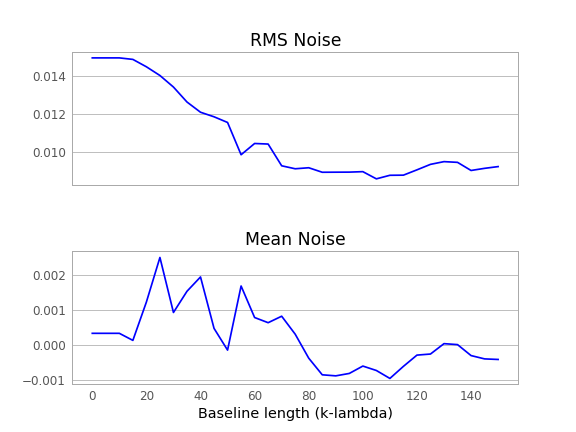
\includegraphics[width=.6\linewidth]{hcn-imnoise_hcn10000.png}
  \captionof{figure}{First moment map of HCO+, with and without (below and above, respectively) baseline cuts.}
  \label{fig:test1}
\end{minipage}%
\begin{minipage}{.5\textwidth}
  \centering
  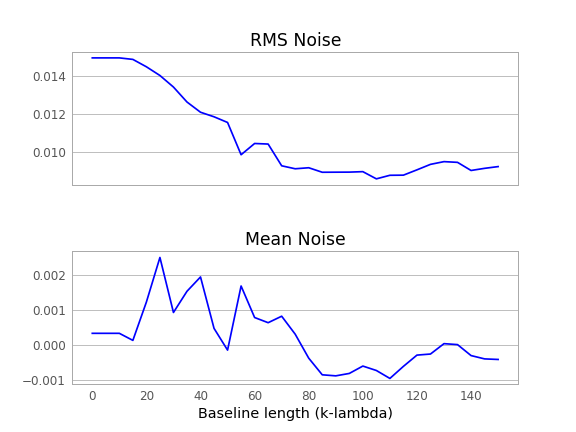
\includegraphics[width=.6\linewidth]{hcn-imnoise_hcn10000.png}
  \captionof{figure}{First moment map of HCN, with and without (below and above, respectively) baseline cuts.}
  \label{fig:test2}
\end{minipage}
\end{figure}

\iffalse
\bigskip
\begin{tabular}{l*{6}{c}r}
  Line                       & HCO$^{+}$ & HCN    & CO    & CS  \\
  \hline
  Min Baseline (k$\lambda$)  &  110      & 80     & 60    & 24.23 (None excluded) \\
  Largest Angular Scale (")  &  1.87     & 2.57   & 3.44  & 8.12 \\
  Angular Resolution (")     &  0.45     & 0.45  & 0.47   & 0.47 \\
\end{tabular}

\bigskip
\bigskip
\fi


\bigskip
\bigskip
\textbf{probably don't need angular res here}
\begin{tabular}{l*{6}{c}r}
  Line       & \shortstack{Baselines \\ (")} & \shortstack{Max Angular Scale \\ (")} & Angular Resolution & \shortstack{Integrated Line Flux \\ (Jy km s$^{-1}$)} \\
  \hline
  \hline
  CS (7-6)         & All                            & 8."5 & 0."47 \\
  CO (3-2)         & All                            & 8."4 & 0."47 \\
  CO (3-2)         & \textgreater 60 k$\lambda$     & 3."4 & 0."47 \\
  HCN (4-3)        & All                            & 8."2 & 0."45 \\
  HCN (4-3)        & \textgreater 80 k$\lambda$     & 2."6 & 0."45 \\
  HCO$^{+}$ (4-3)  & All                            & 8."2 & 0."45 \\
  HCO$^{+}$ (4-3)  & \textgreater 110 k$\lambda$    & 1."9 & 0."45 \\
  \hline
\end{tabular}
\caption{Table 1: Integrated Flux Measurements}
\bigskip
\bigskip


\begin{figure}
  \centering
  \includegraphics[height=0.8\textheight]{Noise-copmarison-HCO+_mom0.pdf}
  \caption{blah}
\end{figure}

The effects of these exclusions are detailed in Table 1 and demonstrated on the HCO$^{+}$ line in Figure 1. (Analysis of these plots, bottom of p.3 in Factor et al)


In all lines, rotation of each disk is clearly visible as a transition from red-shifted emission in one corner to blue-shifted emission in the other corner***. The maximum extent of the 3-$\sigma$ contours along the disks' major axes correspond to outer diameters of the HCO+ disks of A and B; outer diameters of the HCN disks of A and B; and outer diameters of the CO disks of A and B, all at a distance of 389pc. The CS emission is not detected strongly enough to provide a reliable measurement (check that this is true)

Tables 2 and 3 present the velocity-integrated line fluxes and the best-fit parameters for a simple elliptical Gaussian fit to the visibilities for each disk, respectively. Integrated line flux was measured using the MIRIAD task cgcurs to integrate the intensity in the zeroth-moment map throughout the region enclosed by the 3 $\sigma$ contour level. Uncertainties in the integrated line flux do not include the 10\% absolute flux calibration uncertainty inherent in the ALMA observations caused by uncertainties int he models of solar system objects used as flux callibrators. Elliptical Gaussian fits of the visibilities were performed using the MIRIAD task uvfit.

Assuming optically thin emission (maybe good?) and Local Thermodynamic Equilibrium (LTE), the line-emitting gas mass, M$_{\text{gas}}$ is given by:

\begin{align}
  M_{\text{gas}}= \frac{4 \pi}{h \nu_0} \frac{F m d^2}{A_{ul} X_u},
\end{align}

where $F$ is the integrated line flux, $m$ is the mass of the emitting gas molecule, $d$ is the distance to the source, $h$ is the Planck constant, $\nu_0$ is the molecular line's rest frequency, $A_{ul}$ is the Einstein coefficient for the ($u - l$) transition, and

\begin{align}
  X_u = \frac{N_u}{N_{\text{tot}}} = (2 J_u + 1) \frac{\exp [-B_0 J_u (J_u + 1) h c/kT_{\text{ex}}]}{kT_{\text{ex}}/hc B_0}.
\end{align}

In (2), $\frac{N_u}{N_{\text{tot}}}$ is the ratio of the number of molecules in the upper state to the total number of molecules; $J_u$ is the quantum number of the upper level; $B_0$ is the rotation constant in units of wavenumber; $h$ and $c$ are the Planck constant and speed of light, respectively; and $T_{\text{ex}}$ is the excitation temperature. VALUES FOR A_UL AND B0 WERE TAKEN FROM MOLECULAR DATA MADE AVAILABLE BY SHOIER ET AL 2005. LOTS MORE TO DO HERE.


A position-velocity diagram for HCO$^{+}$ is shown in Figure 4, showing the position, as a function of velocity, of emission form a cut along the major axis of the disk (FIGURE OUT HOW TO DO THIS).
ANALYSIS of this stuff.




To find best fit values, we use disk modeling and ray-tracing code developed by \citet{flaherty2013}. The code turns a set of paramters describing the disk's physical structure (atmospheric temperature, density structure, molecular abundances, and so on) into a three dimensional model. Given observational characteristics (distance, inclination, and so on), it can then turn that model into a simulated sky-projected image which may then be compared to our observational data.

Explorations of paramter space were implemented through



Things to get:
* Rewrite this whole thing.
* Previous observation of these disks with SMA? Maybe Mann & Williams 2009. What did they detect?
* Integrated Flux Measurements
* Make a 2-image subplot of HCO+ with and without baseline cutting. Moment 0 or Moment 1? Show n-sigma contours
  * Find max width of disks for each line by 3-sigma contour

* Make moment0 and moment1 plotters. Two panel or just 1? Should have contouring.
* Use cgcurs to get integrated line flux in moment0 map.
* use uvfit for elliptical guassian vis fits.
* PV Diagram
* Gas mass calculations





% Note that no closing info is needed.
